% -*- coding: utf-8 -*-

\chapter{Integración}\label{ch:integracion}

El funcionamiento del sistema requiere la integración de sus distintos componentes. El robot debe combinar su capacidad para localizarse correctamente en el entorno con el seguimiento de una trayectoria adecuada, resultante de la planificación y el control reactivo. La localización resulta imprescindible para el buen funcionamiento del control y, particularmente, para detectar situaciones en que el robot quede alejado de la trayectoria definida (como en la figura \ref{fg:reg}%
%\footnote{Página \pageref{fg:reg}}%
).

La interacción entre el módulo de localización y el de control de movimiento se lleva a cabo mediante la clase \prog{CRobot}, como puede apreciarse en el diagrama \ref{fg:uml}.%
%\footnote{Página \pageref{fg:uml}}
Desde las clases \prog{CRobotGLWnd} y \prog{CControl3GUIDlg} se realiza la transferencia de información desde la interfaz gráfica al resto del programa. En esta última se tiene el objeto \prog{gl_wnd}, de la clase \prog{CRobotGLWnd}, el objeto \prog{robot}, de la clase \prog{CRobot} y el objeto \prog{control}, de la clase \prog{CMoveControl}. Desde \prog{robot} se tiene un puntero al objeto \prog{control}. Desde \prog{gl_wnd} se tienen punteros a  \prog{robot} y a \prog{control} (para simplificar las llamadas a sus métodos y no tener que utilizarlos a través del puntero al objeto \prog{robot}).

\section{La clase \texttt{CRobot}}
El papel de esta clase consiste en integrar:
\begin{itemize}
  \item la obtención de los datos de odometría y del láser
  \item la estimación o/y corrección de la posición mediante el filtro de Kalman y la actualización del mapa
  \item el paso de la posición corregida y del mapa de obstáculos al módulo de control de movimiento
\end{itemize}
Para ello se dispone de algunas variables miembro importantes:
\begin{itemize}
  \item \prog{robotdata}, de la clase \prog{CRobotDataReal}
  \item \prog {proc_laser_data}, de la clase \prog{CProc_Laser_Data}
  \item \prog{loc}, de la clase \prog{CKalman_Loc}
  \item \prog{control}, puntero a un objeto de la clase \prog{CMoveControl} (que habrá de apuntar al objeto \prog{control} miembro del diálogo \prog{CControl3GUIDlg}).
\end{itemize}
%\noindent
También posee una variable puntero a un objeto de tipo \prog{CPioneer}, para las pruebas de control que se han hecho con el robot P3AT.

%Las funciones que forman parte de la clase son las siguientes:

%\subsection{SetPioneer}
%
%\noindent
%\prog{void SetPioneer(CPioneer* pioner)}
%
%\noindent
%Esta función se emplea para hacer que el puntero miembro de \prog{CRobot} apunte a un objeto \prog{CPioneer} determinado que se le pasa como parámetro.
%
%\begin{itemize}
%  \item \prog{pioner}: puntero al objeto de la clase \prog{CPioneer} al que se quiere apuntar desde un objeto \prog{CRobot}.
%\end{itemize}
%
%\subsection{SetControl}
%
%\noindent
%\prog{void SetControl(CMoveControl* cont)}
%
%\noindent
%Esta función se utiliza para hacer que el puntero miembro de \prog{CRobot} apunte a un objeto \prog{CMoveControl} determinado que se le pasa como parámetro.
%
%\begin{itemize}
%  \item \prog{cont}: puntero al objeto de la clase \prog{CMoveControl} al que se quiere apuntar desde un objeto \prog{CRobot}.
%\end{itemize}
%
%\subsection{shutdown}
%
%\noindent
%\prog{void shutdown()}
%
%\noindent
%Esta función sirve para desconectar el robot Pioneer en caso de que se esté utilizando.

\subsection{\texttt{ProcessData}}

\noindent
\prog{int ProcessData()}

\noindent
Es la función principal de la clase. Sirve para integrar los componentes que se han indicado anteriormente.

\noindent
En primer lugar se actualizan los datos odométricos y del láser mediante \prog{robotdata.UpdateData()}.

Si se han obtenido datos de la odometría (valor de retorno \prog{ODOM_DATA} o \prog{DATA_ODOM_LASER}) se calcula el incremento que ha de utilizarse para la etapa de predicción del algoritmo de localización a partir de la transformación inversa de la posición odométrica previa y su composición con la posición odométrica recién obtenida. La nueva posición se guarda como posición antigua para la siguiente llamada a la función. En caso de que se haya añadido un ruido adicional (a través del cuadro de diálogo), se inyecta éste en el incremento de odometría mediante composición con aquél. La posición odométrica con el ruido extra se guarda en un vector de la STL para su representación gráfica. Por último se calcula la predicción de la posición odométrica mediante \prog{loc.KalmanPos} con los argumentos correspondientes al incremento de odometría calculado.

Si se han obtenido datos del láser (\prog{robotdata.UpdateData()} ha devuelto \prog{LASER_DATA} o \prog{DATA_ODOM_LASER}) lo primero que se hace es procesar la información del mismo que estará disponible en la variable de la clase \prog{CRawLaserData} perteneciente a \prog{robotdata} para que en \prog{proc_laser_data} se tenga el vector \prog{v} con los puntos correspondientes a las medidas del láser (llamada a \prog{proc_laser_data}.\prog{DefineData}(\prog{robotdata.laser_data}).
Seguidamente se realizan las operaciones necesarias para calcular los puntos del polígono correspondiente a esa serie de medidas del láser mediante el objeto \prog{proc_laser_data}. Se obtienen también los ángulos $\alpha$ de la figura \ref{fg:poligono} y se pasan éstos y la información del polígono a variables miembro del objeto \prog{loc}. Se calcula la corrección de la posición estimada por medio de \prog{loc.KalmanUpdate}, pasándole como argumento el vector \prog{v} de la variable \prog{proc_laser_data}.

La posición resultante de esta actualización se guarda en un vector de la STL para representar en la interfaz gráfica la trayectoria corregida mediante el algoritmo de localización y poder compararla con la trayectoria basada únicamente en los datos de la odometría.

Esta nueva posición es la que ha de utilizar el control de movimiento. Como las variables \prog{x} y \prog{y} de la clase \prog{CMoveControl} son públicas, basta con asignarles el valor correspondiente a la posición corregida con el filtro de Kalman.

Lo último que se hace es pasarle a la variable \prog{control} el vector con aquellos puntos del mapa (actualizado en la llamada a \prog{ KalmanUpdate}) suficientemente cercanos al robot como vector que contiene los obstáculos a evitar por el control reactivo y efectuar la deformación de la trayectoria mediante \prog{control.ComputeElasticTray()}.

El valor de retorno es 1 si se han actualizado datos de odometría o del láser y 0 en caso contrario.

Esta función va a ejecutarse a modo de bucle, dentro de un \emph{timer} que se define en la clase \prog{CControl3GUIDlg}.

\section{La clase \texttt{CControl3GUIDlg}}
Esta clase hereda de la clase pública \prog{CDialog}, perteneciente a las MFC. En ella comienza el hilo principal de ejecución del programa. Desde esta clase se crea el cuadro de diálogo, al que han de añadirse los diferentes botones para realizar el paso de información del usuario a los distintos componentes del sistema. En ella se tiene la variable \prog{gl_wnd} para crear la ventana gráfica y asociarla a él. Como se ha mencionado, proporciona el modo de controlar el ciclo de tareas que ha de realizar el robot mediante un temporizador o \emph{timer} que permite la repetición de una serie de acciones periódicamente. La variable \prog{robot}, de acuerdo con lo visto, es necesaria para obtener la posición corregida y el mapa y hacer posible su utilización desde el control de movimiento en cada momento. La variable \prog{control} se emplea para facilitar el acceso a aquél. %Las principales funciones editadas en esta clase son:

\section{Interfaz de usuario}
Aunque ya se ha mostrado en otras figuras, a continuación se presenta el aspecto final de la interfaz de usuario desarrollada (figura \ref{fg:interfaz}). En esta imagen se ve tal y como aparece al iniciarse la ejecución del programa (salvo los colores de fondo y cuadrícula, que por defecto son negro y magenta pero pueden cambiarse pulsando en el teclado la letra 'F'). Seguidamente se describirán sus propiedades y la utilidad de sus botones.

\begin{figure}[h]
  % Requires \usepackage{graphicx}
  \centering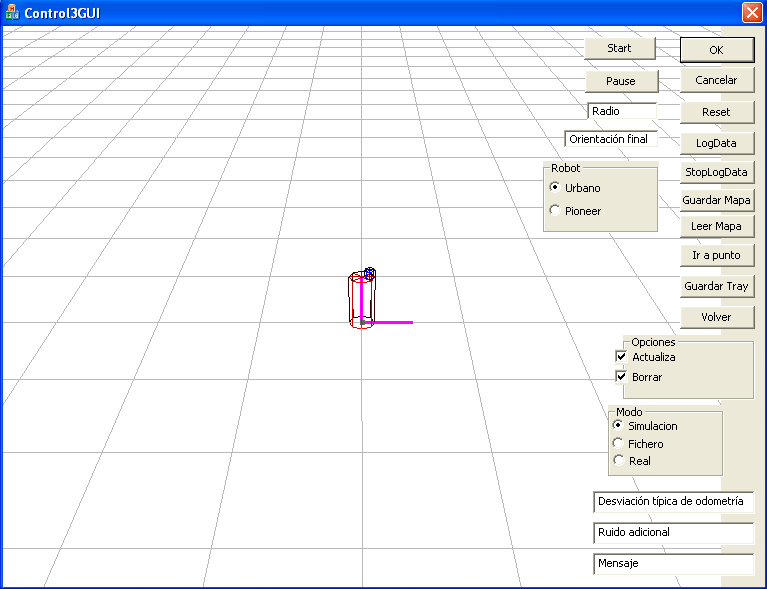
\includegraphics[scale=0.4]{interfazNueva}\\
  \caption{Interfaz de usuario}\label{fg:interfaz}
\end{figure}


\subsection{Funcionalidad de los botones del diálogo}\label{botones}

\subsubsection{OK y Cancelar}

%\noindent
Siempre que se pulse alguno de estos botones se cierra la interfaz de usuario y finaliza la ejecución del programa.

\subsubsection{Reset}
%\noindent
Se emplea para anular la definición de una trayectoria y de una serie de obstáculos realizados mediante el ratón.

\subsubsection{Guardar Mapa}

%\noindent
Se utiliza para guardar los puntos de un mapa en un fichero. Ha de ser pulsado tras finalizar el recorrido del robot por el entorno que se desee representar. Al ser marcado se abre el típico cuadro de Windows \emph{Guardar Como} para seleccionar el directorio y el nombre del fichero. De esta forma, no tienen que realizarse nuevos mapas cada vez sino que pueden ser leídos mediante \emph{Leer mapa}:

\subsubsection{LeerMapa}

%\noindent
Muestra un cuadro de Windows tipo \emph{Abrir} para establecer como mapa los puntos leídos de un fichero creado mediante \emph{Guardar Mapa}.

\subsubsection{Ir a punto}

%\noindent
Se emplea para que el robot siga una trayectoria definida sobre la interfaz gráfica mediante el ratón.

\subsubsection{Guardar Tray}

\noindent
Permite guardar la trayectoria que sigue el robot, para que luego pueda regresar al punto de partida. Ha de pulsarse en el momento en que se desee que empiece a guardarse el camino, normalmente antes de que comience el movimiento del robot.

\subsubsection{Volver}

%\noindent
Cuando se pulsa este botón el robot emprende el camino de regreso por la misma trayectoria seguida hasta el momento.

\subsubsection{Opciones}
Dentro de este grupo de botones de tipo \emph{check-box} se ofrecen algunas alternativas de funcionamiento del sistema:
\begin{itemize}
  \item Actualiza: permite añadir o no puntos al mapa en función de las medidas del láser. Si no se ha leído ningún mapa mediante \emph{Leer Mapa} y no se marca esta opción, el mapa permanecerá vacío y no podrá efectuarse la localización. Puede variarse la condición elegida a lo largo del funcionamiento del sistema.
  \item Borrar: sirve para establecer si se han de borrar los puntos dinámicos mediante el algoritmo del polígono envolvente o no. En caso afirmativo se dibuja sobre la pantalla el polígono correspondiente en cada momento y los puntos que han sido borrados aparecen en color cyan.
\end{itemize}

\subsubsection{Modo}
Este grupo de botones \emph{radio-box} se emplea para seleccionar el tipo de conexión que se desea.
\begin{itemize}
  \item Simulación: establece el funcionamiento del sistema en modo simulación
  \item Fichero: establece el funcionamiento del sistema en modo fichero
  \item Real: establece el funcionamiento del sistema en modo real
\end{itemize}

\subsubsection{LogData}
Permite guardar en un fichero los datos de odometría y del láser mediante la llamada al método \prog{StartLogData} de la clase \prog{CRobotData}.

\subsubsection{StopLogData}
Se utiliza para cerrar el fichero anterior y de este modo dejar de registrar los datos. Básicamente realiza una llamada a \prog{StopLogData} de la clase \prog{CRobotData}.

%\vspace{0.2cm}
%\noindent
\paragraph{Nota:}
Lógicamente, los dos botones anteriores no se encuentran activados si el modo de funcionamiento es tipo fichero.

\subsubsection{Desviación típica de odometría}
En esta \emph{edit box} puede introducirse el valor de la desviación típica en los datos de la odometría que se ha de utilizar en el filtro de Kalman. Si en ella no se escribe ningún valor, se emplea una desviación típica de 0.1.

\subsubsection{Ruido adicional}
El valor que se introduzca en esta \emph{edit box} será inyectado como ruido adicional a la odometría. Permite evaluar el funcionamiento del algoritmo de localización con distintas calidades de los datos odométricos. Si no se escribe nada en el cuadro, el valor por defecto es 0.

\subsubsection{Mensaje}
En esta \emph{edit box} se muestra información sobre la última acción que se le ha pedido que realice al robot (\emph{Guardando trayectoria}, \emph{Siguiendo trayectoria})...

\subsubsection{Start}
Con este botón se inicia un temporizador para que se ejecute el ciclo de tareas del robot cada cierto tiempo (periodo de 10ms en los modos simulación y fichero y de 150ms en modo real). Conviene utilizarlo una vez se han seleccionado los parámetros de funcionamiento.

\subsubsection{Pause}
Este botón mata el temporizador y con ello dejan de realizarse las actualizaciones del ciclo, por lo que el sistema se mantiene estático hasta que vuelva a lanzarse el ciclo de tareas pulsando de nuevo el botón \emph{Start}.

\subsubsection{Radio}
El valor que se introduzca en esta \emph{edit box} se utilizará como radio de curvatura para suavizar la trayectoria. Si no se escribe nada en ella el valor por defecto es 1m.

\subsubsection{Orientación final}
Esta \emph{edit box} se utiliza si se desea concretar una orientación del robot en el punto final de la trayectoria. Si se ha pulsado la opción de \emph{Volver} la orientación final será por defecto la que tenía el robot en el momento en que se comenzó a guardar la trayectoria. En caso contrario el robot mantendrá la orientación con la que llegue al destino.

\subsubsection{Robot}
Este grupo de botones se utiliza para escoger el tipo de robot que se va a emplear.
\begin{itemize}
  \item Urbano: opciones correspondientes al robot Urbano (B21r de iRobot).
  \item Pioneer: opciones correspondientes al robot Pioneer (P3AT de ActivMedia Robotics).
\end{itemize}

Las principales diferencias entre seleccionar uno u otro robot se hallan en el modo en que se realiza la conexión, en la forma en que se envían los comandos de velocidad y se recibe la información de la odometría y del láser y en los parámetros del control de movimiento. La separación de ambos casos se realiza, por lo tanto, en las clases \prog{CControl3GUIDlg} (conexión en el botón \emph{Start} y envío de comandos en el \emph{timer}), \prog{CRobot} (obtención de las medidas del sistema odométrico y de las observaciones proporcionadas por el láser) y \prog{CMoveControl} (regulador para seguir la trayectoria).

\subsection{Selección de opciones mediante ratón o teclado} \label{opciones}
Por medio del ratón pueden realizarse los siguientes cambios relativos a la visualización:
\begin{itemize}
  \item Acercamiento y alejamiento del punto de vista mediante giro de la rueda del ratón en uno u otro sentido. El mismo resultado se obtiene moviendo el ratón con el botón derecho pulsado.
  \item Variación del punto de vista manteniendo apretado el botón izquierdo del ratón mientras se mueve.
  \item Desplazamiento del origen de coordenadas del sistema de referencia global sobre el plano representado en la interfaz gráfica pulsando simultáneamente el botón izquierdo del ratón y el botón \emph{Ctrl} del teclado y arrastrando el cursor.
  \item Desplazamiento del origen de coordenadas de sistema global sobre el eje z del mismo al mover el ratón y mantener pulsados el botón derecho y la tecla \emph{Ctrl}.
  \item Creación y representación de obstáculos mediante doble click con el botón izquierdo del teclado. Si existe una trayectoria definida esta acción provoca la deformación de la misma.
  \item Definición de puntos de una trayectoria. Si no se trata del primer punto de la misma, se obtiene la trayectoria redondeada inmediatamente después de haberse añadido el nuevo punto.
\end{itemize}

A través del uso único del teclado pueden hacerse más modificaciones:
\begin{itemize}
  \item Cambio del tipo de representación de 2D a 3D y viceversa con la tecla correspondiente a la letra 'P'
  \item Cambio del color del fondo y algunos otros colores con la tecla correspondiente a la letra 'F'
  \item Ocultar o mostrar la cuadrícula que muestra el plano del movimiento con la tecla correspondiente a la letra 'G'
  \item Mostrar o no mostrar la trayectoria definida, la trayectoria modificada y los obstáculos mediante las teclas correspondientes a las letras 'T', 'E' y 'O' respectivamente
  \item Aumentar y disminuir el tamaño de las celdas de la cuadrícula por medio de las teclas correspondientes a las letras 'M' y 'L'
  \item Movimiento del robot en modo teleoperado. La letra 'W' se utiliza para aumentar la velocidad de avance; la 'S', para disminuir la velocidad de avance; la 'D', para incrementar la velocidad de giro (sentido de las agujas del reloj, figura \ref{fg:velocidades}); la 'A' para disminuir la velocidad de giro (o incrementarla en sentido antihorario) y la barra de espaciado se emplea para hacer nulas las velocidades del robot y que éste se detenga.
\end{itemize}

\section{Pruebas y resultados}
En estas pruebas se pone de manifiesto la interacción entre las dos partes principales del sistema desarrollado.

\subsection{Pruebas en modo \emph{simulación}}
Como ya se ha visto, en este modo de funcionamiento no se realiza localización del robot por no haber disponibilidad de medidas del láser para el robot Urbano. Sin embargo, sí que permite evaluar la deformación de trayectorias en entornos densos en obstáculos mediante el uso de mapas.

\subsubsection{Movimiento sobre trayectoria deformada ante los obstáculos definidos por los puntos de un mapa}
A continuación se utilizan mapas obtenidos por los métodos descritos en el capítulo \ref{ch:localizacion} de modo que sus puntos sean los que sirvan para deformar la trayectoria. La trayectoria inicial se dibuja en color azul y la deformada, en color verde. Se ha tomado un rango de 1m a la posición del robot para considerar los puntos del mapa como obstáculos. La máxima desviación permitida se ha establecido en 0.3m para evitar deformaciones excesivas y no entrar en situación de bloqueo con demasiada facilidad.%Se puede ver que con una desviación máxima de 0.6m la trayectoria deformada (dibujada en color verde), se corta antes de que termine la trayectoria inicial (color azul), lo que significa que se ha producido bloqueo.

\begin{figure}[htb]
  \centering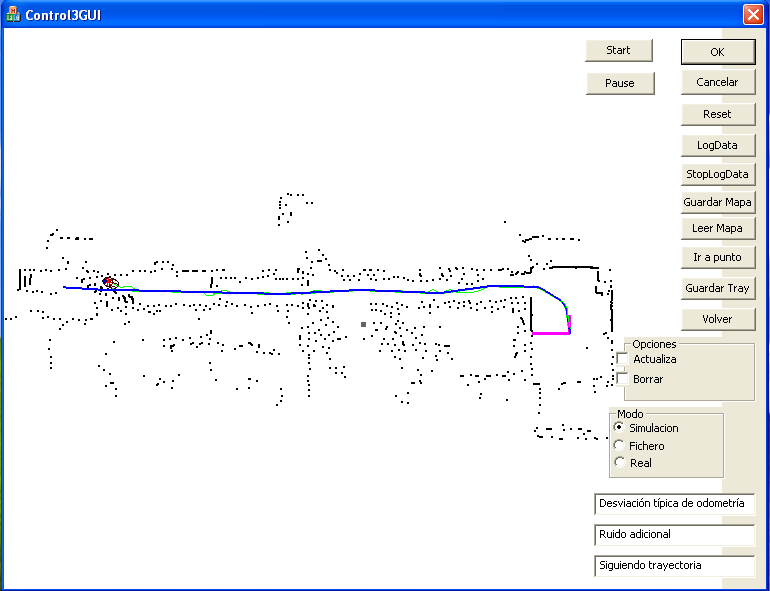
\includegraphics[scale=0.8]{reactivo1}
   \caption{Deformación de trayectorias definidas en el laboratorio de DISAM-UPM (a)}\label{fg:react3a}
\end{figure}

\begin{figure}[htb]
  \centering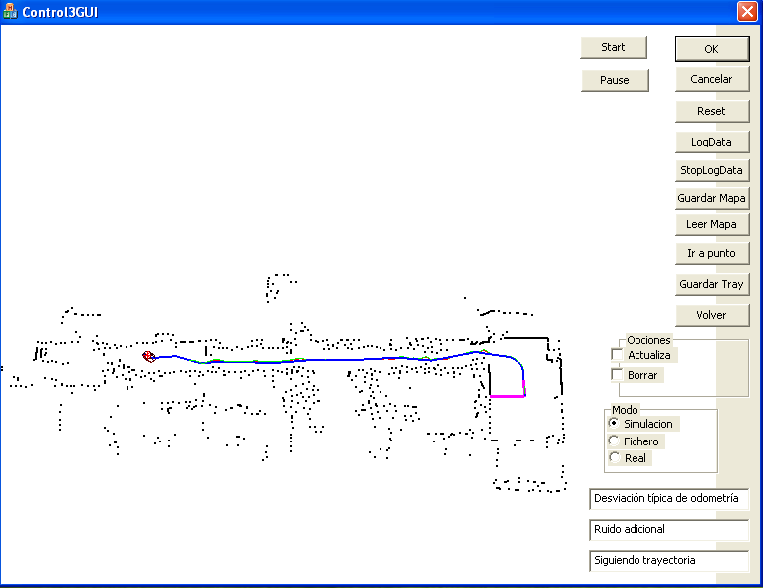
\includegraphics[scale=0.7]{reactivo2}
  \caption{Deformación de trayectorias definidas en el laboratorio de DISAM-UPM (b)}\label{fg:react3b}
\end{figure}

\clearpage
Aquí puede verse la utilidad del borrado de puntos dinámicos del mapa. En \ref{fg:react3a}, hay obstáculos que impiden el avance del robot en una cierta zona (situación de bloqueo). Dichos obstáculos, sin embargo, no son puntos reales del mapa sino que corresponden probablemente a sucesivas posiciones de una persona en el momento de la toma de datos. Si el mapa hubiera sido obtenido con la opción de borrado activada, como resultaría conveniente, el robot podría llegar hasta el final del recorrido planificado (figura \ref{fg:react3c}).

El número de obstáculos considerados en este tipo de situaciones es significativamente alto, por lo que la trayectoria deformada difiere de la original. En caso de que se desee que el robot regrese al punto de origen de su movimiento se empleará como trayectoria nominal sobre la que realizar los cambios oportunos la trayectoria seguida en el camino de ida, siendo ésta una trayectoria deformada en base a la trayectoria nominal inicial. En la figura \ref{fg:reactVuelta} se muestra en color azul la trayectoria seguida durante la ida (trayectoria nominal del camino de vuelta) y en color rosa la trayectoria modificada durante el camino de regreso, tras la aparición de un nuevo obstáculo.

\begin{figure}[hb]
  % Requires \usepackage{graphicx}
  \centering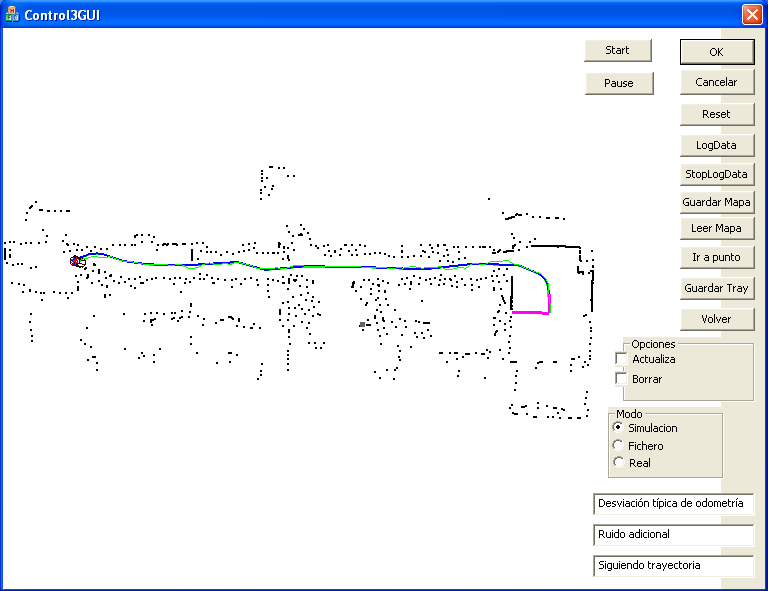
\includegraphics[scale=0.9]{reactivo3}
  \caption{Deformación de trayectorias en un mapa obtenido con borrado de puntos dinámicos}\label{fg:react3c}
\end{figure}

\begin{figure}[h]
  % Requires \usepackage{graphicx}
  \centering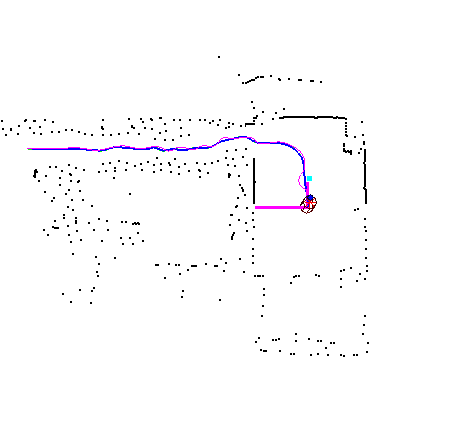
\includegraphics[scale=0.8]{reactVuelta}\\
  \caption{Trayectoria deformada en el camino de ida y nuevas deformaciones en el camino de vuelta}\label{fg:reactVuelta}
\end{figure}

\clearpage

\subsubsection{Construcción de un mapa mediante movimiento controlado del robot y deformación de la trayectoria ante los puntos del mismo con el robot Pioneer}

Con este robot, el simulador proporcionado por el fabricante permite disponer de las medidas ficticias del láser en un entorno hipotético representado en el mismo por medio de un mapa geométrico de líneas. Así, puede verse el comportamiento del sistema desarrollado a la hora de construir el mapa de puntos de un entorno como el dado por aquél mapa. En la figura \ref{fg:pioneerSim1a} se muestran los resultados de un primer experimento. En ella pueden apreciarse algunos detalles interesantes.

\begin{figure}[h]
  % Requires \usepackage{graphicx}
  \centering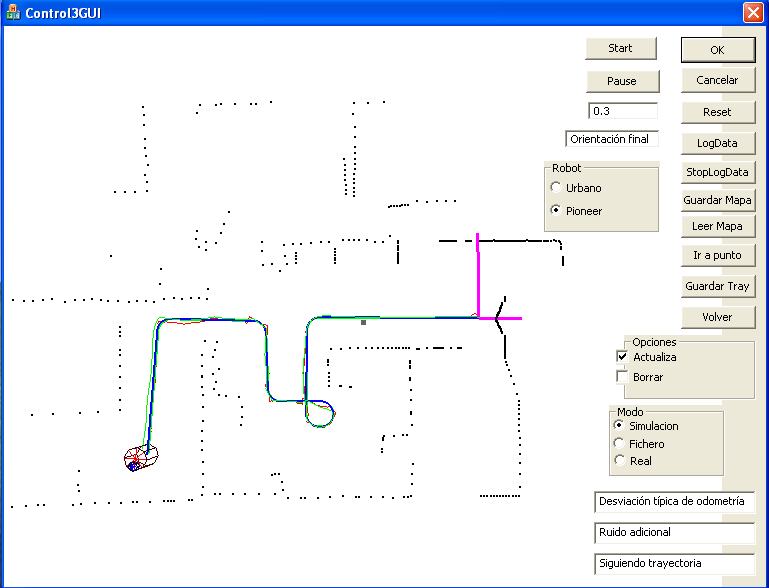
\includegraphics[scale=0.4]{pioneer3}

  \vspace{0.5cm}

  \centering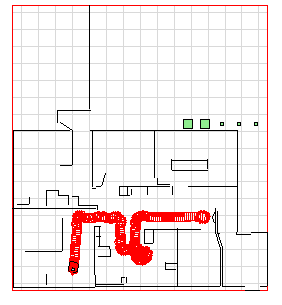
\includegraphics[scale=0.7]{pioneer3_sim}
  \caption{Primer experimento para ver el comportamiento del sistema con el robot Pioneer}\label{fg:pioneerSim1a}
\end{figure}

 Como primera conclusión podría destacarse la insuficiencia de un valor de 0.1 en la estimación del ruido de la odometría, lo que afecta a la construcción del mapa y hace que se creen paredes dobles en algunos casos. La posición corregida por el filtro aparece en color rojo, mientras que la de la odometría es la que se dibuja en color verde. Al final del recorrido empieza a apreciarse la desviación en la posición odométrica. La trayectoria azul es la nominal, definida por el usuario mediante el ratón, y la trayectoria deformada no se muestra, pero es bastante similar a la trayectoria real seguida(trayectoria roja). Puede verse que se deforma adecuadamente en los puntos cercanos a las paredes o muebles.

 En un segundo experimento (figura \ref{fg:pioneerSim1b}) se mejoró la estimación del ruido de la odometría (estableciéndose en un valor de 0.5), con lo que aumenta la calidad del mapa construido. Posiblemente se obtendrían mejores resultados incrementando algo más dicho valor. Los colores empleados son los mismos que en el caso anterior, pero sólo se representa el último tramo de la trayectoria nominal definida. De nuevo se puede observar la deformación de la trayectoria en las cercanías de los obstáculos y el efecto de la localización, más fácilmente apreciable en observación simultánea en tiempo real de ambos simuladores.

 \begin{figure}[h]
  % Requires \usepackage{graphicx}
  \centering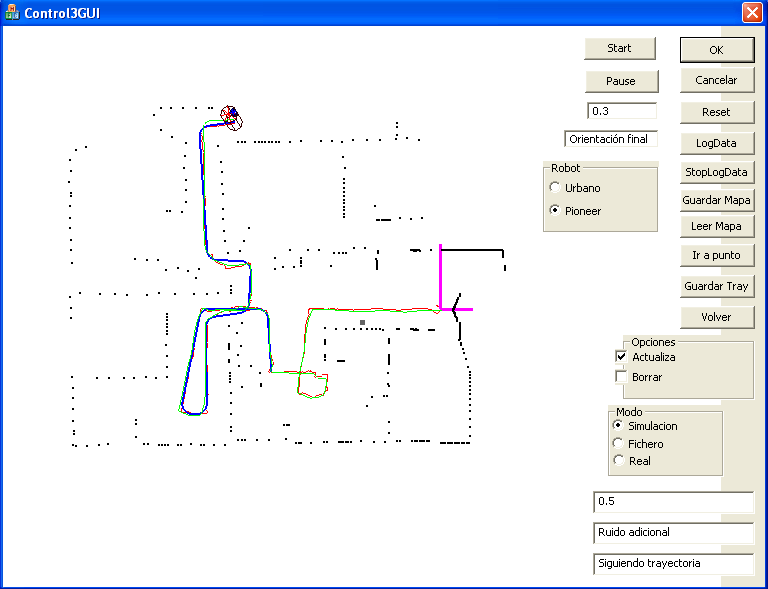
\includegraphics[scale=0.4]{pioneer2}

  \vspace{0.5cm}

  \centering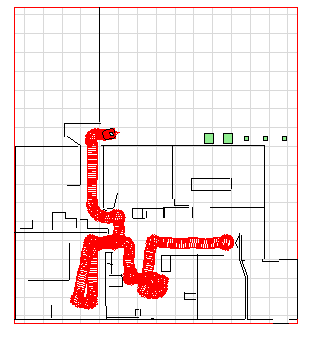
\includegraphics[scale=0.62]{pioneer2_sim}
  \caption{Segundo experimento para ver el comportamiento del sistema con el robot Pioneer}\label{fg:pioneerSim1b}
\end{figure}

\clearpage
\subsection{Pruebas en modo \emph{real}}

En la figura \ref{fg:RealMapa1} se puede ver la trayectoria deformada seguida por el robot al acercarse a un perchero situado en una esquina del laboratorio. A medida que iba siguiendo dicha trayectoria planificada se iba actualizando el mapa. El valor de la desviación típica del ruido considerado para la odometría (0.1 por defecto)probablemente es escaso, pero la longitud del recorrido no es suficiente para apreciarlo. La orientación de partida del robot no era paralela a las paredes, lo que hace menos intuitiva la interpretación de resultados. Las desviaciones observadas en la trayectoria seguida fueron corregidas mediante las modificaciones en el control de movimiento descritas en \ref{control} y plasmadas en el cuadro \ref{vel2}.

\begin{figure}[h]
  % Requires \usepackage{graphicx}
  \centering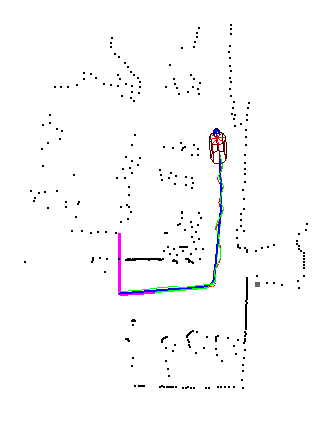
\includegraphics[scale=0.7]{RealMapa}\\
  \caption{ Primer experimento del sistema conjunto en modo real}\label{fg:RealMapa1}
\end{figure}

En un segundo experimento, figura \ref{fg:RealMapa2}, pasaron varias personas por la zona de detección del láser. La mayor parte de los puntos correspondientes fueron borrados, como puede observarse. La trayectoria seguida resultó ser algo más suave en este caso. La estimación de la desviación típica del ruido en las medidas de odometría ($\sigma_{odom} = 0.3$) parece ser más correcta; aunque los errores de este tipo son menores de lo esperado y la trayectoria odométrica resulta ser bastante aproximada a la real.

\begin{figure}[h]
  % Requires \usepackage{graphicx}
  \centering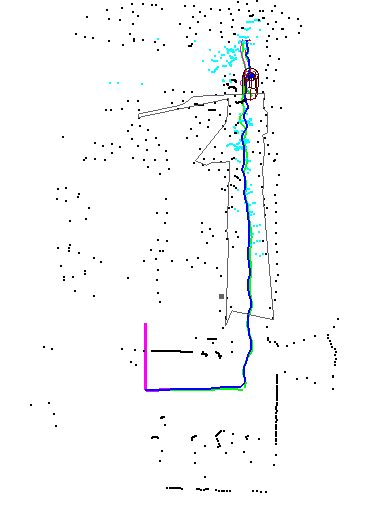
\includegraphics[scale=0.65]{RealMapa2}\\
  \caption{ Segundo experimento del sistema conjunto en modo real}\label{fg:RealMapa2}
\end{figure}

%\clearpage
Una tercera prueba consistió en llevar al robot en modo teleoperado hasta el final del laboratorio y hacer que regresara al punto inicial de manera autónoma. Los resultados se muestran en la figura \ref{fg:LaboRealVuelta}. La trayectoria dibujada en color azul es la trayectoria real seguida por el robot durante la ida y la dibujada en rojo (superpuesta con la anterior, apenas distinguible dado que no hubo cambios en el entorno que afectaran a puntos lo suficientemente cercanos al robot como para ser considerados como obstáculos) es la real correspondiente al camino de vuelta. En color verde se representa la trayectoria odométrica de la ida y en color magenta, la odometría de la vuelta. El valor de $\sigma_{odom}$ tomado es nuevamente 0.3; se vio en el capítulo \ref{ch:localizacion} que un valor de 0.5 en general resulta más apropiado.

\begin{figure}[h]
  % Requires \usepackage{graphicx}
  \centering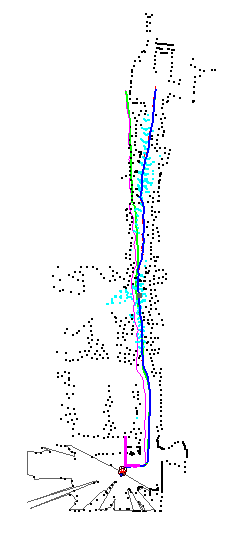
\includegraphics[scale=0.8]{LaboRealVuelta}\\
  \caption{ Tercer experimento del sistema conjunto en modo real}\label{fg:LaboRealVuelta}
\end{figure} 